\documentclass{article}
\usepackage{polyglossia}

\usepackage{xcolor}
\definecolor{links}{HTML}{2A1B81}
\usepackage{hyperref}
\hypersetup{
    pdfencoding=auto,
    pdftitle={GSOC_2019 KM3NeT project challenge},
    pdfauthor={Roel Aaij},
    pdfcreator={LaTeX},
    pdfproducer={LuaTex 1.0.4},
    colorlinks,
    linkcolor=,
    urlcolor=links
}
\usepackage[export]{adjustbox}
\usepackage{graphicx}
\usepackage{amsmath}
\usepackage{amsthm}
\usepackage{wasysym}
\usepackage{pict2e}
\usepackage{ifthen}
\usepackage{listings}
\usepackage[left=2.5cm, right=2.5cm, top=2.5cm]{geometry}

\usepackage{fontspec}
\usepackage{unicode-math}
\setsansfont[Ligatures=TeX]{Linux Biolinum O}
\setmathfont{Latin Modern Math}
\setmathfont[range=\mathit/{latin,Latin,num,Greek,greek}]{Linux Biolinum O Italic}
\setmathfont[range=\mathup/{latin,Latin,num,Greek,greek}]{Linux Biolinum O}
\setmathfont[range=\mathbfup/{latin,Latin,num,Greek,greek}]{Linux Biolinum O Bold}
\setmathfont[range={"221E}]{Linux Biolinum O}% "0221E = \infty

\usepackage{caption}
\captionsetup{labelformat=empty,labelsep=none}

\lstset{language=C++,
  keywordstyle=\color{blue},
  stringstyle=\color{red},
  commentstyle=\color{green},
  morecomment=[l][\color{magenta}]{\#}
}
\lstMakeShortInline[columns=fixed]|

\title{Challenge for GSoC 2019 Project on Speeding up KM3NeT's Reconstruction}
\author{Roel Aaij}

\begin{document}

\section{Description of KM3NeT}

\begin{figure}
  \center
  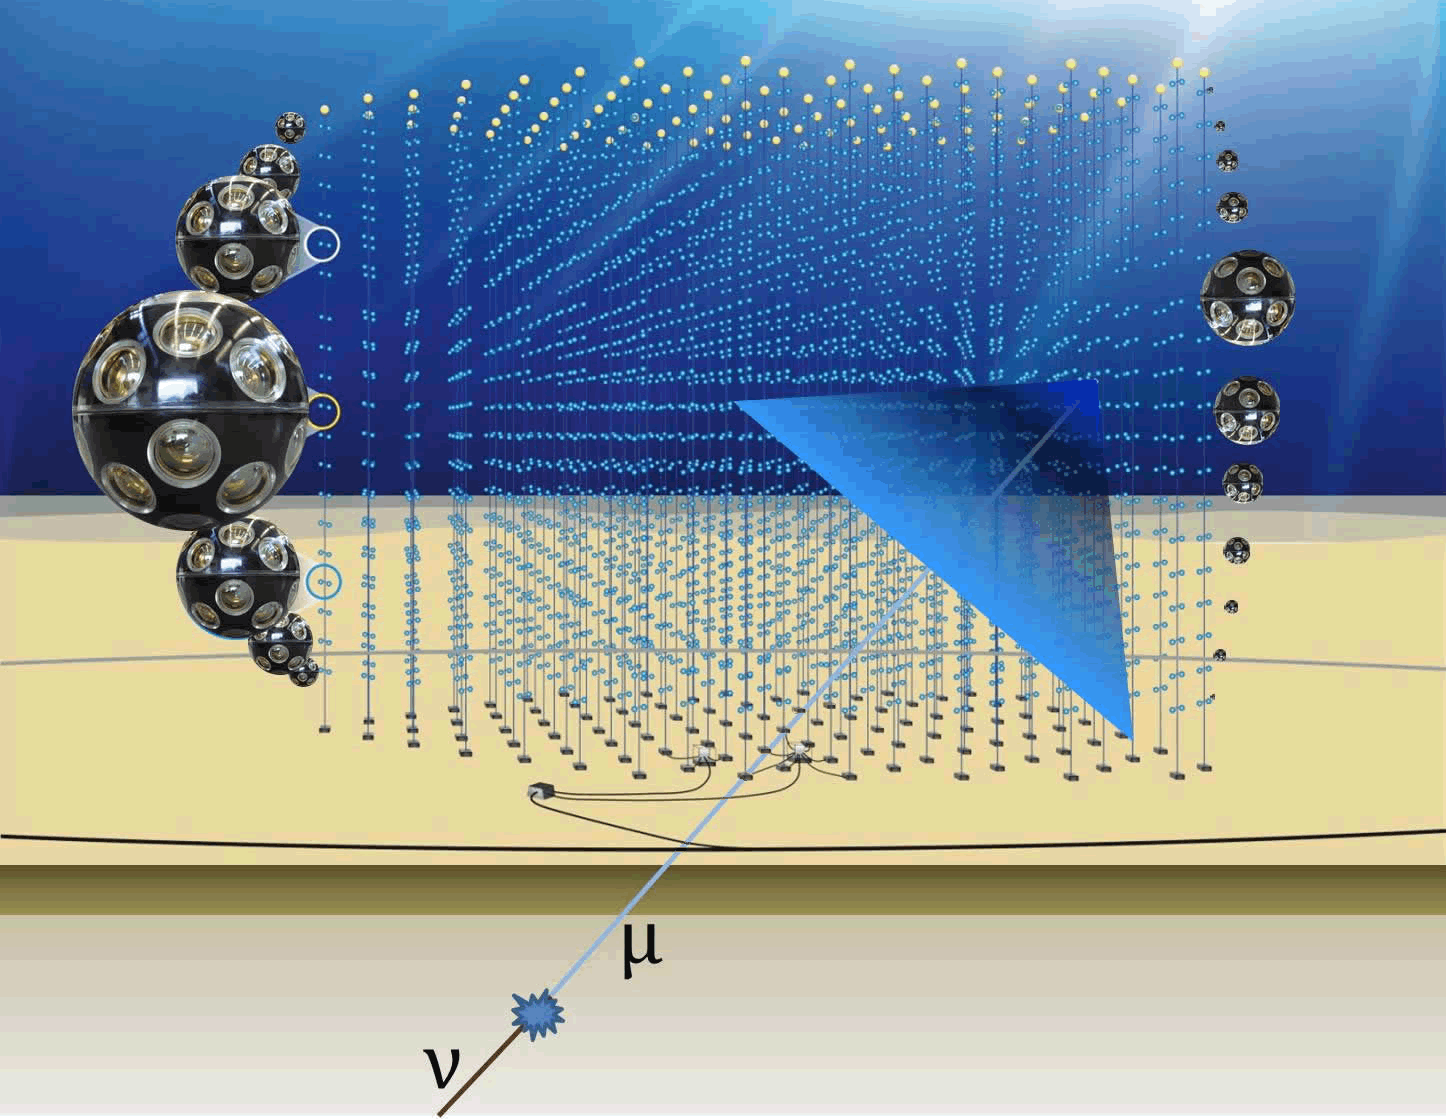
\includegraphics[width=0.6\textwidth]{KM3NeT-NeutrinoToMuon.png}
  \caption{A muon traversing the KM3NeT detector}
\end{figure}

KM3NeT is an underwater research facility that houses two large
neutrino telescopes: ORCA and ARCA. The ORCA telescope consists of a
number of strings (MOD) of optical modules (DOM) attached to the floor
of the Mediterranean Sea off the coast of Toulon in France.

The optical modules each contain 31 photomultiplier tubes (PMTs) that
detect light emitted by muons and electrons that traverse water inside
the detector. Some of these muons and electrons are created by
interactions of neutrinos with the water or sea floor. These are the
muons and electrons that KM3NeT aims to detect and whose trajectory
and energy it aims to reconstruct.

\section{Background Generator Library}

There are also several other sources of light present in the water,
which create so-called background noise. A standalone generator that
simulates such noise is available at
\href{https://github.com/nlesc-km3net/k40gen}{https://github.com/nlesc-km3net/k40gen}. The
k40gen package also houses this challenge.

\section{Challenge}

The C++17 code for this challenge is available on the GSoC\_2019
branch of the k40gen repository. It consists of a skeleton file
containing |main| that needs to be completed. The file can be found in
the ``challenge'' subdirectory. Please stick to C++17 (or an earlier
standard) to implement this challenge.

\subsection{Part 1}

The file |km3net_reference.detx| in the ``challenge'' subdirectory of
the repository contains a reference geometry of the detector. Part 1
of the challenge aims to parse this file into some form of storage for
usage later in the program.

The first three lines of |km3net_reference.detx| can be ignored. The
fourth line contains the number of strings in the detector. The rest
of the file consists of information about the optical modules that the
strings consist of. The first optical module (DOM) section starts at
the fifth line. DOM sections are separated by a blank line.

Each optical module section starts with a line that consists of 4
numbers: the |DOM_ID|, the |MOD_ID|, the number of the DOM within the
MOD, and the number of PMTs in this DOM. The a single line for each
PMT follows which consists of: unique |PMT_ID|, X position, Y
position, Z position, X direction, Y direction, Z direction and a
calibration constant. The positions are in meters and the directions
together form a unit vector. The calibration constant is not relevant
for this challenge.

\subsection{Part 2}

The second part of the challenge aims to randomly select a range of
hits to be used for part 3. It is suggested to use a flat distribution
to select the first hits, and a normal distribution with a mean of 20
and a width of 5 to select the number of additional hits.

\subsection{Part 3}

The 3rd part of the challenge is about rotating the directions of the
PMTs of the hits selected in part 2, and storing the result of the
rotation for later reference. This part has two sub-parts: A and B.

\subsubsection{Part 3A}

Please write down the math you propose to implement to rotate the PMTs
over two angles: $\theta$ and $\phi$, where $\theta$ is the polar
angle of a system of spherical coordinates with its zenith direction
along the z-axis, and $\phi$ is the azimuthal angle in the same
system.

\subsubsection{Part 3B}

It is suggested to implement two functions that do the work of the
rotation, first to obtain the parameters of the rotation from the
angles $\theta$ and $\phi$, and another to apply the rotation to the
direction of the PMTs selected in part 2.

\section{Testing}

To test whether the code works, it is suggested to also implement the
inverse of the functions that are used to obtain and apply the
rotations: obtaining and applying the inverse of a rotation,
$R_{-1}$, after $R$ has been applied should return a PMT to it's
original position.

\section{Bonus}

As a bonus, briefly discuss implementing the rotations using AVX2
vector instructions. A brief discussion on optimal data structures for
use with a vectorized implementation is also welcome.

\section{Notes and Dependencies}

The k40gen package is implemented in C++17 and uses CMake as its build
system. Python bindings for the |generate(...)| function are also available,
but are probably less relevant to this challenge. They can be disabled
at build time by passing \verb|-DENABLE_PYTHON=FALSE| to cmake when
configuring.

\subsection{C++17}
The package requires a C++17-compliant compiler and standard library
to build it.

\subsection{Range V3}
The skeleton provided for this challenge uses the RangeV3 library —
\href{https://github.com/ericniebler/range-v3}{https://github.com/ericniebler/range-v3}
— to sort the generated |PMT_IDs| according to their timestamp. It is
assumed to be installed on the build system. If not, it can be
installed separately, but the CMake files would have to be updated to
properly include it.

\subsection{Vc}
The Vc library —
\href{https://github.com/VcDevel/Vc}{https://github.com/VcDevel/Vc} —
is used to implement an AVX2 version of the generator, and is
downloaded and built by CMake if not available on the system.

\section{Submitting}

Please submit your completed challenge by mail to the mentors as a
tarball of relevant files or a single patch to the GSOC\_2019 branch of
the k40gen repository.

\section{Questions and Contact}

Please address questions by mail to the mentors:
\begin{itemize}
\item \href{mailto:roel.aaij@nikhef.nl}{Roel Aaij}
\item \href{mailto:rbruijn@nikhef.nl}{Ronald Bruijn}
\item \href{mailto:m.de.jong@nikhef.nl}{Maarten de Jong}
\end{itemize}

\noindent Best of luck!

\end{document}
